\subsubsection{Plasmonic gratings considered in \cite{pendry2016acsphotonics} behaving as bianisotropic metamaterial}
In  \cite{pendry2016acsphotonics}, Kraft et. al consider a plasmonic grating 
which exhibits bianisotropy at visible wavelength.
Here we consider scattering problems involving an equivalent medium 
that can be characterized by the constitutive matrices of the same form 
given in the paper.
The region occupied by the scatterer may be denoted as $\Omega_s \subset \Omega$. 
We start with the form of the normalized constitutive relation as found in 
\cite{chen2005retrieval} and \cite{li2009determination}, 
and obtain the $P$, $Q$, $L$, $M$ matrices \cite{noiregolarita}.
The final form given below is obtained by considering 
non magnetic material with 
$\mu_r=1$ and with an isotropic complex relative permittivity $\varepsilon_r$. 
The magnetoelectric coupling parameter is denoted $\zeta_0$. 

\begin{equation}  \label{constitutive_kraft_P}
P = c_0 \varepsilon_0 
\begin{bmatrix}
\varepsilon_r & 0 & 0 \\
0 &  \varepsilon_r & 0 \\
0 & 0 & \varepsilon_r-\zeta_0^2
\end{bmatrix} 
\end{equation}

\begin{equation} \label{constitutive_kraft_Q}
Q = \frac{1}{c_0\mu_0}I
\end{equation}

\begin{equation} \label{constitutive_kraft_LM}
L = M^T = \frac{j\zeta_0}{\mu_0 c_0}
\begin{bmatrix}
0 & 0 & 0 \\
0 & 0 & 0 \\
0 &  1  & 0
\end{bmatrix} 
\end{equation}
 
The complementary region $\Omega \setminus \Omega_s$ is 
occupied by the empty space, which,  in our notation, is characterized by 
 $P=c_0\varepsilon_0I_3$, $Q=\frac{1}{c_0\mu_0}I_3$, $L=M=0$.

The bianisotropic medium is lossy with the imaginary part $Im(\varepsilon_r) < 0$, 
where as $\zeta_0$ is assumed real here to avoid some longer calculation. 
Now Lemma 1 of \cite{kalarickel2020well} can be applied to verify hypothesis H5.
Inside $\Omega_s$, $P$ can be decomposed as $P= P_s -j P_{ss}$ with
\begin{equation}
P_s = \frac{P+P^*}{2} =  c_0\varepsilon_0
\begin{bmatrix}
Re(\varepsilon_r) & 0 & 0 \\
0 & Re(\varepsilon_r) & 0 \\
0 & 0 & Re(\varepsilon_r) - \zeta_0^2 \\
\end{bmatrix},
\end{equation}
and  $P_{ss} = \frac{P^*-P}{2j} =  -c_0\varepsilon_0 Im(\varepsilon_r) I_3$.
Hence we have $\Omega_{el} = \Omega_s$, the lossy region 
where $P_{ss}$ is uniformly positive definite 
and the complementary region with free space where $P_s$ 
is uniformly positive definite.
This means that the conditions of relevant Lemma are satisfied and 
as a result H5 is valid.

From the definitions
$C_1=c_0\varepsilon_0 |Im(\varepsilon_r)|$, 
$C_2 = c_0\varepsilon_0$ and 
$C_3 = c_0\varepsilon_0 \max(|Re(\varepsilon_r) -\zeta_0^2|, |Re(\varepsilon_r)|)$.
To find the minimum of the two expressions in \eqref{eq:cps_metamaterial},
we note that, in the valid range, the value of the 
first expression decreases monotonically with  $\alpha$ where as
that of the second expression increases with it. 
The highest estimate for $C_{PS}$  is obtained when the two expressions 
have the same value.
The value of $\alpha$ at which this happens can be evaluated by 
equating the two expressions and finding the positive 
root of the resulting quadratic equation.
This value of $\alpha$, denoted as $\alpha_{opt}$ is given by 
\eqref{eq:alpha_opt}.

\begin{equation}  \label{eq:alpha_opt}
\alpha_{opt} = \frac{C_2^2-C_1^2-C_3^2 + \sqrt{(C_2^2-C_1^2-C_3^2)^2+4C_2^2C_3^2}}{2C_2^2}
\end{equation}

Thus we may simply write 
\begin{equation} \label{eq:cps_metamaterial_optimal}
C_{PS} = \sqrt{\frac{1-\alpha_{opt}}{2}}c_0\varepsilon_0.
\end{equation}
As mentioned before, this does not mean that a better value of $C_{PS}$ 
cannot be found.
For example, if $Re(\varepsilon_r) -\frac{\zeta_0^2}{\mu_r} > 0$, 
then $P_s$ is uniformly positive definite in $\Omega$ and we can find 
another candidate for $C_{PS}$, namely $C_4 = c_0\varepsilon_0\min(1, |Re(\varepsilon_r-)\zeta_0^2|$.
In particular, when  $Re(\varepsilon_r) - \zeta_0^2 > 1$, $C_4 = c_0\varepsilon_0$ is always going to give a value for $C_{PS}$ which is higher than that obtained from the Lemma.

The generality of out theory be clearly demonstrated by showing its 
applicability to bianisotropic metamaterials. 
Hence in the rest of the subsection the discussion  focuses on 
the cases with $\varepsilon_r < 0$.
For this case,$C_3 = c_0\varepsilon_0 |Re(\varepsilon_r) -\zeta_0^2|$ , and we can directly use the value of $C_{PS}$ in \eqref{eq:cps_metamaterial_optimal}.
Since the material is assumed to be non magnetic the direct application of definition 
gives $C_{QS} = \frac{1}{c_0\mu_0}$.
Likewise, the continuity constants $C_L = C_M = \frac{|\zeta_0|}{c_0\mu_0}$.
Then the inequality in H7 becomes $C_{QS} -\frac{C_L C_M}{C_{PS}} = \frac{1}{c_0\mu_0}(1 -\frac{\zeta_0^2\sqrt{2}}{\sqrt{1-\alpha_{opt}}}) > 0$, 
which gives \eqref{eq:inequality_zeta0}.

\begin{equation} \label{eq:inequality_zeta0}
|\zeta_0| < \left(\frac{1 - \alpha_{opt}}{2}\right)^{1/4}.
\end{equation}

Since the right hand side of \eqref{eq:inequality_zeta0} also depends on 
$\zeta_0$ due to the presence of $C_3$ in the expression for $\alpha_{opt}$,
we do not have a closed form expression on the limit on $\zeta_0$ 
below which H7 is satisfied.
However a graphical analysis can be done for estimating such a limit 
on $|\zeta_0|$, as shown in 
Figure \ref{fi:critical_zeta_vs_epsilonr_inf_sup}.
The value of $Re(\varepsilon_r)$ is varied in the range $(-1.0,-5.0)$ 
whereas $Im(\varepsilon_r)$ assumes values in the range $(-0.1,-0.5)$.
It can be observed that for a fixed value of $Im(\varepsilon_r)$, 
the range of $\zeta_0$ over which H7 is valid steadily decreases as 
$|Re(\varepsilon_r)|$ increases. 
As for the dependence on $Im(\varepsilon_r)$, the corresponding range
increases when medium becomes more lossy due to higher $|Im(\varepsilon_r)|$,
as expected.

\begin{figure}[H]
\centering
\begin{subfigure}[b]{0.49\textwidth}
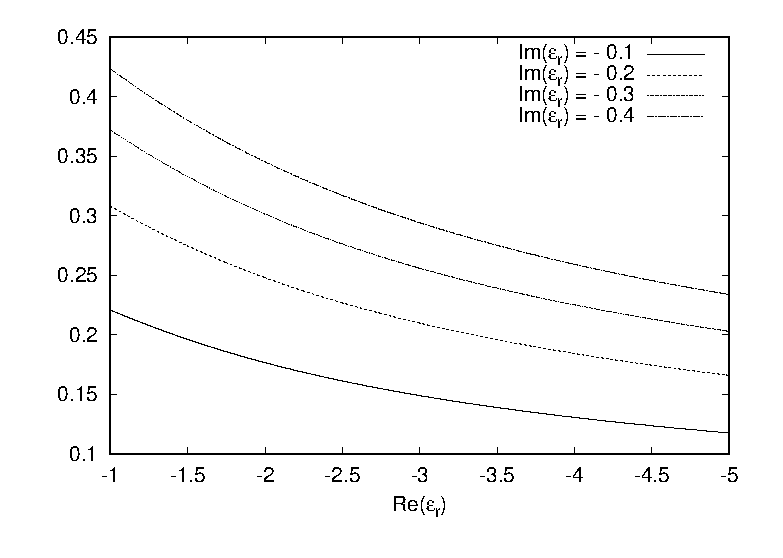
\includegraphics[width=\textwidth]{critical_zeta_vs_real_epsilon_pendry_inf_sup.eps}
\end{subfigure}
%
\begin{subfigure}[b]{0.49\textwidth}
\centering
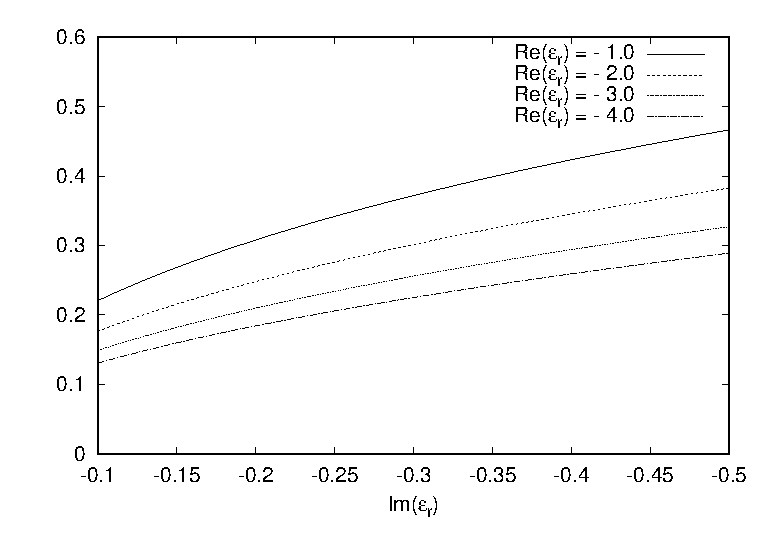
\includegraphics[width=\textwidth]{critical_zeta_vs_imag_epsilon_pendry_inf_sup.eps}
\end{subfigure}
\caption{The magnitude of $|\zeta_0|$ below which the condition \ref{eq:infsup} is satisfied as a function of $Re(\varepsilon_r)$ or $Im(\varepsilon_r)$ for media in Kraft et al.
The plot is for real $\zeta_0$ negative values of  $Re(\varepsilon_r)$ or $Im(\varepsilon_r)$ and the material is taken to be non magnetic.}
\label{fi:critical_zeta_vs_epsilonr_inf_sup}
\end{figure}

We consider the alternative form of constitutive relations , 
which for the medium inside $\Omega_s$ becomes as
in equations \eqref{constitutive_kraft_kappa} to \eqref{constitutive_kraft_chi_gamma}, 
for examining the validity of H1-H4 \cite{noiregolarita}.

\begin{equation} \label{constitutive_kraft_kappa}
\kappa = \frac{1}{\varepsilon_0\varepsilon_r}
\begin{bmatrix}
1 & 0 & 0 \\
0 & 1 & 0 \\
0 & 0 & \frac{\varepsilon_r}{\varepsilon_r-\zeta_0^2}
\end{bmatrix}
\end{equation}

\begin{equation} \label{constitutive_kraft_nu}
\nu = \frac{1}{\mu_0}
\begin{bmatrix}
1 & 0 & 0 \\
0 & \frac{\varepsilon_r}{\varepsilon_r - \zeta_0^2} & 0 \\
0 & 0 & 1
\end{bmatrix}
\end{equation}

\begin{equation} \label{constitutive_kraft_chi_gamma}
\gamma = -\chi^T = \frac{j\zeta_0c_0}{\varepsilon_r-\zeta_0^2}
\begin{bmatrix}
0 & 0 & 0 \\
0 & 0 & 1 \\
0 & 0 & 0
\end{bmatrix}
\end{equation}

Since H1-H4 needs to hold only locally, and they are trivially 
valid in the empty space outside the bianisotropic media, 
we have to just analyze them inside $\Omega_s$ occupied by the bianisotropic medium.
These constants can be evaluated directly from the definitions. 
The determinants of $\kappa$ and $\nu$ are, respectively, 
$\frac{1}{(\varepsilon_0 \varepsilon_r)^3(1-\frac{\zeta_0^2}{\varepsilon_r})}$ and
$\frac{1}{(\mu_0)^3(1-\frac{\zeta_0^2}{\varepsilon_r})}$  which immediately give the values of  $C_{\kappa,d}$ and $C_{\nu,d}$.

\begin{equation}
C_{\kappa,d} =  \frac{1}{|\varepsilon_0^3\varepsilon_r^3(1 - \frac{\zeta_0^2}{\varepsilon_r})|}, 
\end{equation}

\begin{equation}
C_{\nu,d} =  \frac{1}{|\mu_0^3(1 - \frac{\zeta_0^2}{\varepsilon_r})|}.
\end{equation}

The inverses of the diagonal matrices $\kappa$ and $\nu$ are just the 
diagonal matrices with the reciprocal entries.
Applying equations \eqref{equationnumber35} and \eqref{equationnumber36} gives the values of $C_{\kappa,r}$ and $C_{\nu,r}$.

\begin{equation}
C_{\kappa,r} =  |\varepsilon_0\varepsilon_r (1 - \frac{\zeta_0^2}{\varepsilon_r})|,
\end{equation}

\begin{equation}
C_{\nu,r} =  |\mu_0 (1 - \frac{\zeta_0^2}{\varepsilon_r})|. 
\end{equation}

Using equations \eqref{equationnumber35} and \eqref{equationnumber36} we get the $C_{\kappa,s}$ and $C_{\nu,s}$.

\begin{equation}
C_{\kappa,s} =  \frac{1}{\varepsilon_0} \max(\frac{2}{|\varepsilon_r|}, \frac{1}{|\varepsilon_r|}(1 + \frac{1}{|1 - \frac{\zeta_0^2}{\varepsilon_r}|})),
\end{equation}

\begin{equation}
C_{\nu,s} = \frac{1}{\mu_0} \max(2, (1 + \frac{1}{|1 - \frac{\zeta_0^2}{\varepsilon_r}|})),
\end{equation}

Since we are interested in the case when $Re(\varepsilon_r) < 0$ and real $\zeta_0$, 
 we see that $|1 - \frac{\zeta_0^2}{\varepsilon_r}| > 1$,   and the maximum reduces to 
the values in \eqref{eq:cks_pendry} and \eqref{eq:cnus_pendry}.

\begin{equation} \label{eq:cks_pendry}
C_{\kappa,s} =  \frac{2}{|\varepsilon_0\varepsilon_r|},
\end{equation}

\begin{equation} \label{eq:cnus_pendry}
C_{\nu,s} = \frac{2}{\mu_0}. 
\end{equation}

Using equations \eqref{equationnumber37} and \eqref{equationnumber38} 
we can easily evaluate $C_{\gamma,s}$ and $C_{\chi,s}$. 

\begin{equation}
C_{\gamma,s} =  C_{\chi,s} = |\frac{\zeta_0c_0}{\varepsilon_r - \zeta_0^2}|. 
\end{equation}

Using these constants, the value of $K_u$  can be calculated using equation \eqref{equationnumber39}.
The critical value of $|\zeta_0|$ below which the condition in H4 is satisfied is plotted in Figure \ref{fi:critical_zeta_vs_epsilonr_uniqueness}, 
with respect to either $Re(\varepsilon_r)$ or $Im(\varepsilon_r)$.
The results show that the range of $\zeta_0$ for which H4 holds true increases with the increase in $|Re(\varepsilon_r)|$, 
while it is practically independent of $Im(\varepsilon_r)$.

\begin{figure}[H]
\centering
\begin{subfigure}[b]{0.49\textwidth}
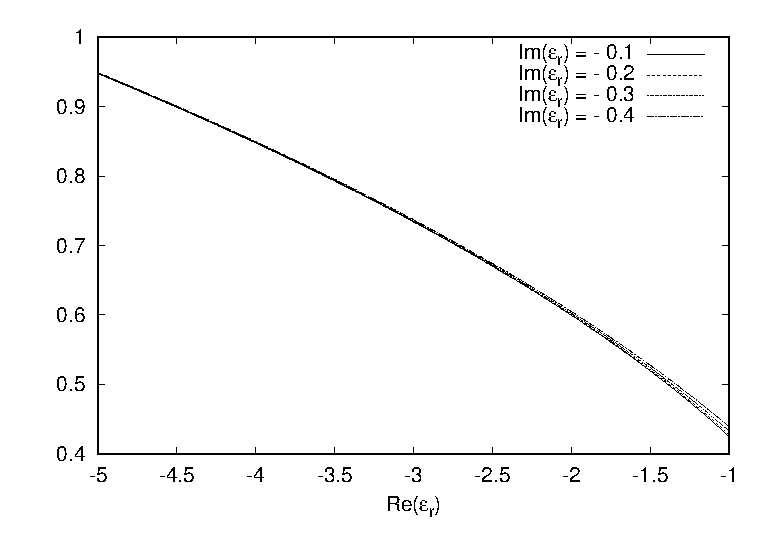
\includegraphics[width=\textwidth]{critical_zeta_vs_real_epsilon_pendry_uniqueness.eps}
\end{subfigure}
%
\begin{subfigure}[b]{0.49\textwidth}
\centering
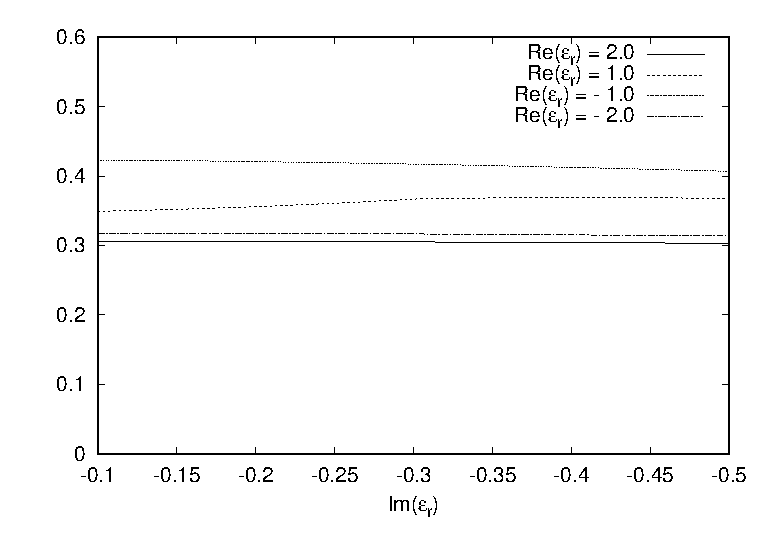
\includegraphics[width=\textwidth]{critical_zeta_vs_imag_epsilon_pendry_uniqueness.eps}
\end{subfigure}
\caption{The magnitude of $\zeta_0$ below which the condition \ref{eq:condizione2diteorema2.22delmonk} is satisfied as a function of $Re(\varepsilon_r)$ or $Im(\varepsilon_r)$ for media in Kraft et al.
The plot is for real $\zeta_0$ and the material is taken to be non magnetic.}
\label{fi:critical_zeta_vs_epsilonr_uniqueness}
\end{figure}

Let us try to understand the implications of the theory by applying it to 
the numerical solution of a specific problem involving the medium of interest.
We consider the region with the scatterer $\Omega_{s}$ to be a cube filled 
with homogeneous bianisotropic media.
The surrounding region is filled with empty space and the overall domain 
of numerical investigation, $\Omega$, is of cubic shape as well, and is 
concentric to $\Omega_{s}$.
In the following $\Omega$ is characterized by sides of length 2 $\mu m$ 
and $\Omega_s$ by those of 0.8 $\mu m$.
The axes are taken along the sides of the cubes and the excitation is 
with a plane wave incident along the x axis, with electric field polarized along 
z axis, having a magnitude of 1 $V/m$ and wavelength of 1 $\mu m$.

Inside $\Omega_s$, the medium is characterized by $\varepsilon_r = -1 - j0.4$, 
$\mu_r = 1$ and $\zeta_0 = -0.41$. 
This value is such that the hypotheses required for well posedness and 
finite element approximability are satisfied.
In fact, for the $\varepsilon_r$ considered, condition \ref{eq:condizione2diteorema2.22delmonk} 
is valid for $|\zeta_0| < 0.4235$ and condition \ref{eq:infsup} is valid for 
$|\zeta_0| < 0.4393$.

The solutions are obtained with a first order edge element based Galerkin 
finite element method. The boundary condition is enforced with $Y$ equal to 
the admittance of vacuum and with an inhomogeneous term ${\bf f}_R$, 
taking into account the incident field. 

The domain is discretized uniformly using tetrahedral meshes.
The meshing is done by first dividing the domain into small identical cubes,
each of which is in turn divided into six tetrahedra.
The parameter $h$ denotes the maximum diameter of all the elements of the 
mesh \cite{handbook} (p. 131), and in this case it is simply given by the side of 
the small cube times $\sqrt{3}$.
To study the convergence of solution, we consider different levels 
of refinement of meshes ranked in order of $h$,
ranging from ``very coarse'' to ``very fine''.
For exmaple the mesh denoted very coarse is characterized by a cubes of sides 
800 nm and the resulting mesh has 1331 nodes, 6000 tetrahedral elements and 
1200 boundary faces.
A summary of the information related to 
the four different refinements of the meshes that was used 
is given in Table \ref{ta:details_about_meshes}.


\begin{table}[H]
  \centering
  
%  \begin{normalsize}
  %
  \begin{tabular}{|c| c| c |c |c |}
    %
    % first horizontal line above the table
    \toprule
    %
    % first line
    %
   \textbf{ Type of Mesh }% column 1
    & \textbf{Maximum Diameter} % column 2
    & \textbf{Number of} % column 3
    &\textbf{ Number of} % column 4
    & \textbf{Number of}\\% column 5
    % new line to introduce a fictitious carriage return
    %\textbf{ Mesh} % column 1
    & \textbf{of the Mesh } % column 2
    & \textbf{Nodes}% column 3
    &\textbf{ Elements} % column 4
    & \textbf{Boundary Faces} \\ % column 5
    % new line to introduce a fictitious carriage return
    % column 1 is empty in this new line
    & \textbf{($h$ in nm)} % column 2; 
    &  % column 3; 
    &  % column 4; 
    & \\ % column 5; 
    %
    \midrule
    %
    % second line
    %
    Very coarse% column 1
    & $200$ $\sqrt{3}$ % column 2
    & $1331$  % column 3
    & $6000$ % column 4
    & $1200$ \\ % column 5
    %\midrule
    Coarse % column 1
    %third line
    & $100$ $\sqrt{3}$% column 2 
    & $9261$ % column 3
    & $48000$ % column 4
    & $4800$\\ % column 5
    %\midrule
    %
    % fourth line
    %
    Fine % column 1
    & $50$ $\sqrt{3}$ % column 2
    & $68921$ % column 3
    & $384000$ % column 4
    & $19200$ \\% column 5
    %\midrule
    %fifth line
     Very fine % column 1
    & $25$ $\sqrt{3}$% column 2
    & $531441$% column 3 
    & $3072000$ % column 4
    & $76800$  \\% column 5
    \bottomrule
  \end{tabular}
  %
%  \end{normalsize}
  \caption{Details of different meshes used.}
  \label{ta:details_about_meshes}
\end{table}
%
The results related to the stability of the simulations are shown in Figure \ref{fi:kraft_pendry_convergence}.
The difference between sucessive refinements progressively decreases 
and the fine and very fine meshes give solution which are stable.
This confirms the well posedness and convergnce result that was predicted 
using the theory.
  
\begin{figure}
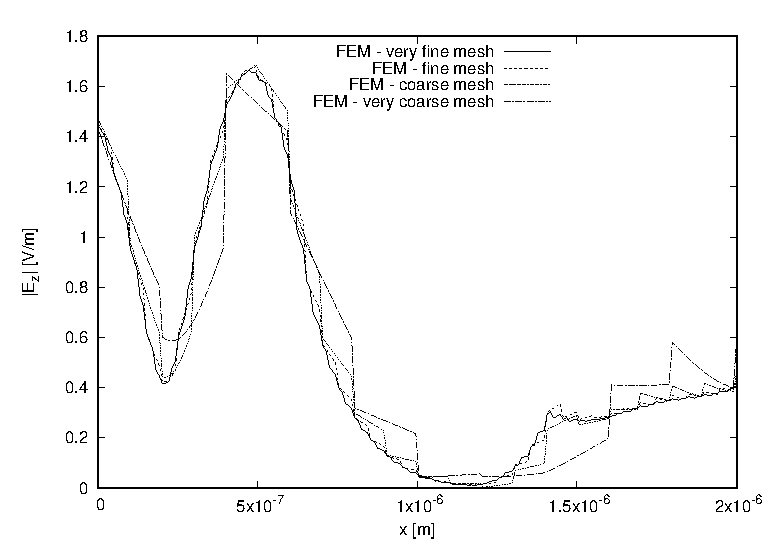
\includegraphics{figure_kraft_pendry_along_x_mag_ez_convergence.eps}
\caption{Convergence of the solution for problem involving medium of Kraft et al.
The magnitude of the $z$ component of the electric field is plotted 
along a line parallel to $x$ axis for four different meshes.}
\label{fi:kraft_pendry_convergence}
\end{figure}

The magnitudes and pahses of some for the components of the field 
along different axis directions are shown in 
Figures  \ref{fi:kraft_pendry_ez_vs_x} to \ref{fi:kraft_pendry_ez_vs_z}.
The solutions obtained for $\zeta_0 = -0.41$ are compared with that 
for the isotropic case ($\zeta_0 = 0$, $\varepsilon_r = -1 -j 0.4$, $\mu_r = 1$).
For example we can see in Figures \ref{fi:kraft_pendry_ez_vs_x} and \ref{fi:kraft_pendry_ez_vs_z}
that there are differences of 10 to 20 percent of the incident field in the 
magnitudes of the electric fields which are induced by the magneto electric coupling 
factor $\zeta_0$.
Likewise the phases of the fields are similarly affected by the bianisotropy of the medium.
These non negligible effects imply that the accuracy of the simulations requires the 
us to consider the bianisotropy of the medium.
Hence the reliability of the finite element silution in the presence of bianisotropy is important 
for getting good results for this kind of problems.
The appliaciton of our theory gives the conditions under which we can guarantee such reliability.


\begin{figure}[H]
\centering
\begin{subfigure}[b]{0.49\textwidth}
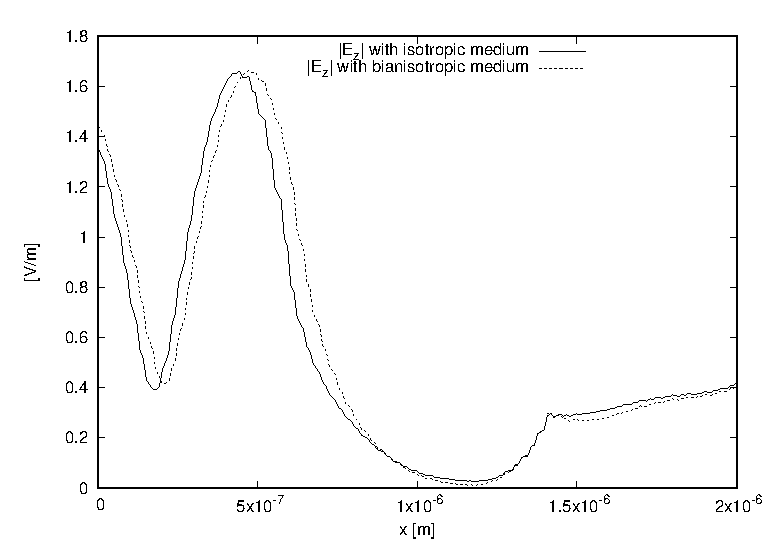
\includegraphics[width=\textwidth]{figure_kraft_pendry_along_x_mag_ez.eps}
\end{subfigure}
%
\begin{subfigure}[b]{0.49\textwidth}
\centering
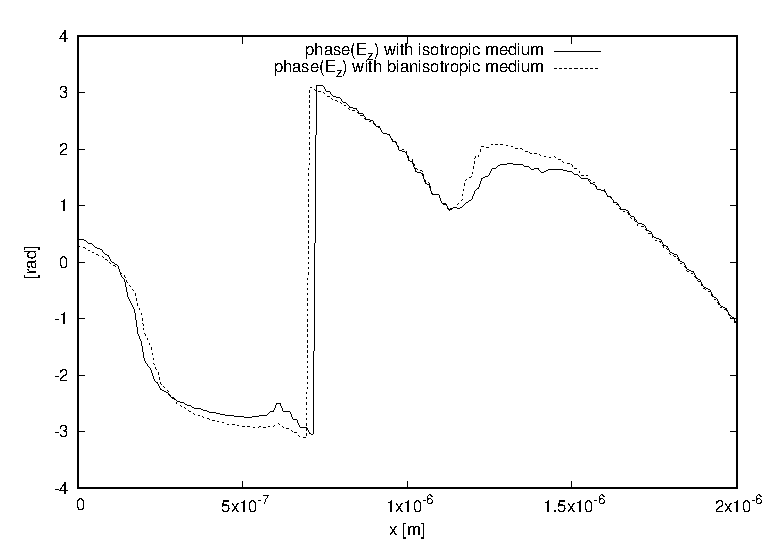
\includegraphics[width=\textwidth]{figure_kraft_pendry_along_x_phase_ez.eps}
\end{subfigure}
\caption{The magnitude and phase of the $z$ component of electric field along a line parallel to $x$ axis 
and passing though the center of gravity of the domain for problem involving medium of Kraft et al. 
The plots for bianisotropic case  using $\zeta_0 = -0.41$ is compared with 
the solution obtained in isotropic case using $\zeta_0 = 0$.}
\label{fi:kraft_pendry_ez_vs_x}
\end{figure}

\begin{figure}[H]
\centering
\begin{subfigure}[b]{0.49\textwidth}
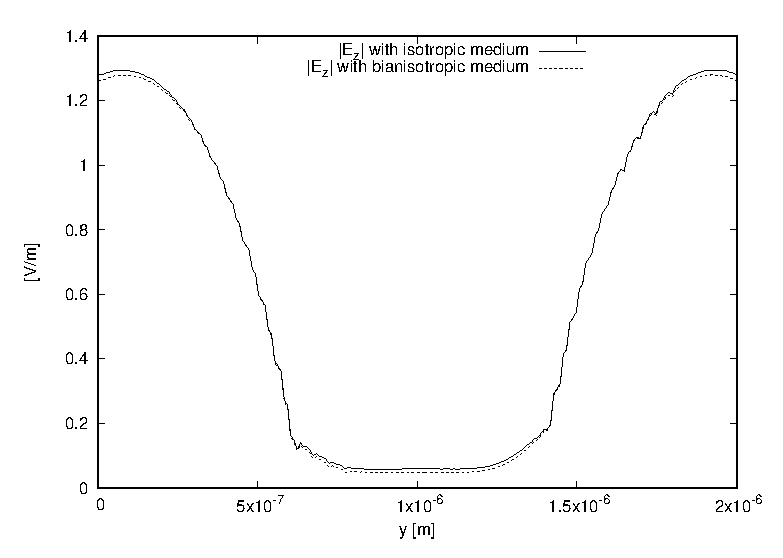
\includegraphics[width=\textwidth]{figure_kraft_pendry_along_y_mag_ez.eps}
\end{subfigure}
%
\begin{subfigure}[b]{0.49\textwidth}
\centering
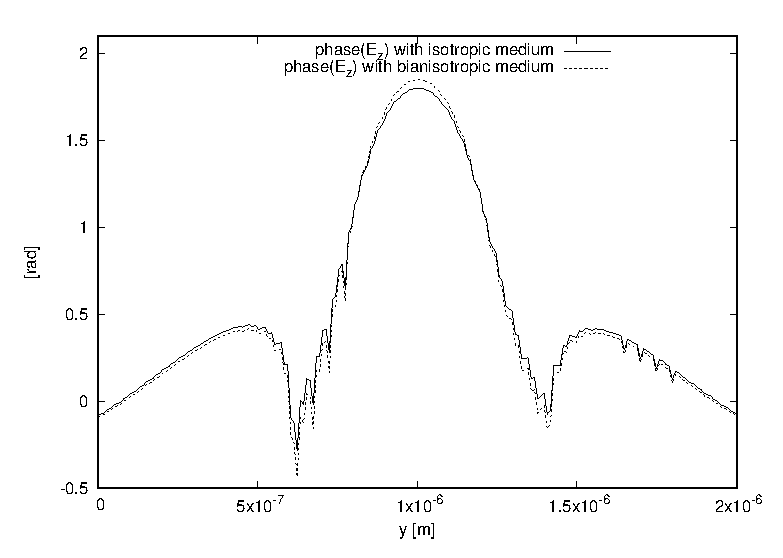
\includegraphics[width=\textwidth]{figure_kraft_pendry_along_y_phase_ez.eps}
\end{subfigure}
\caption{The magnitude and phase of the $z$ component of electric field along a line parallel to $y$ axis 
and passing though the center of gravity of the domain  for problem involving medium of Kraft et al. 
The plots for bianisotropic case using $\zeta_0 = -0.41$ is compared with 
the solution obtained in isotropic case using $\zeta_0 = 0$. }
\label{fi:kraft_pendry_ez_vs_y}
\end{figure}

\begin{figure}[H]
\centering
\begin{subfigure}[b]{0.49\textwidth}
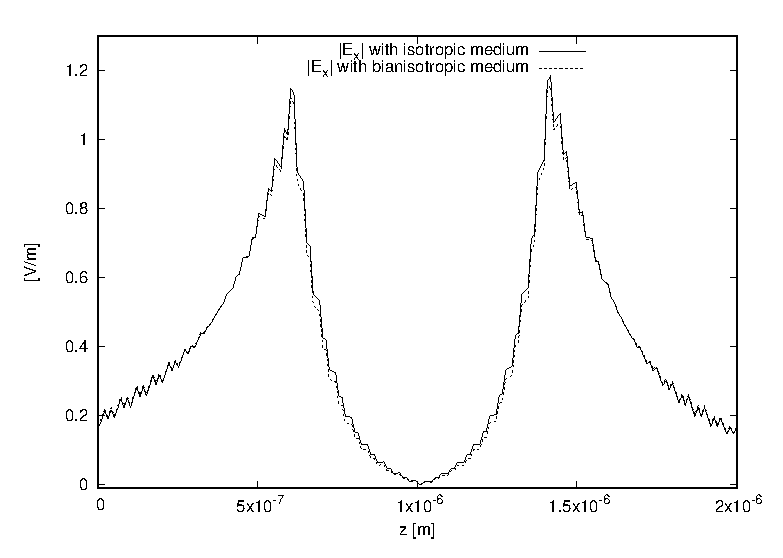
\includegraphics[width=\textwidth]{figure_kraft_pendry_along_z_mag_ex.eps}
\end{subfigure}
%
\begin{subfigure}[b]{0.49\textwidth}
\centering
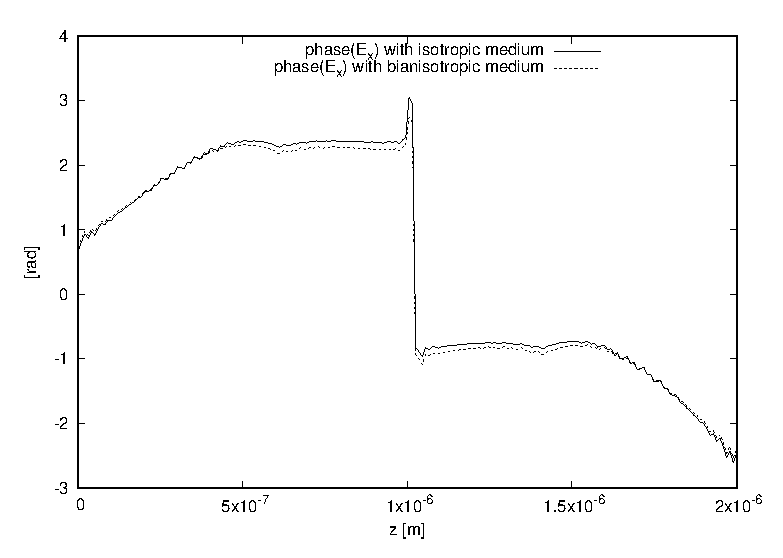
\includegraphics[width=\textwidth]{figure_kraft_pendry_along_z_phase_ex.eps}
\end{subfigure}
\caption{The magnitude and phase of the $x$ component of electric field along a line parallel to $z$ axis 
and passing though the center of gravity of the domain for problem involving medium of Kraft et al. 
The plots for bianisotropic case using $\zeta_0 = -0.41$ is compared with 
the solution obtained in isotropic case using $\zeta_0 = 0$.}
\label{fi:kraft_pendry_ex_vs_z}
\end{figure}

\begin{figure}[H]
\centering
\begin{subfigure}[b]{0.49\textwidth}
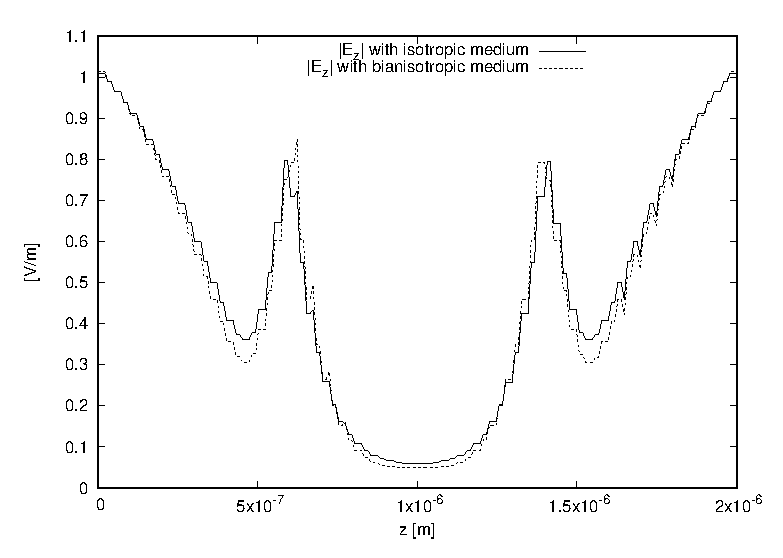
\includegraphics[width=\textwidth]{figure_kraft_pendry_along_z_mag_ez.eps}
\end{subfigure}
%
\begin{subfigure}[b]{0.49\textwidth}
\centering
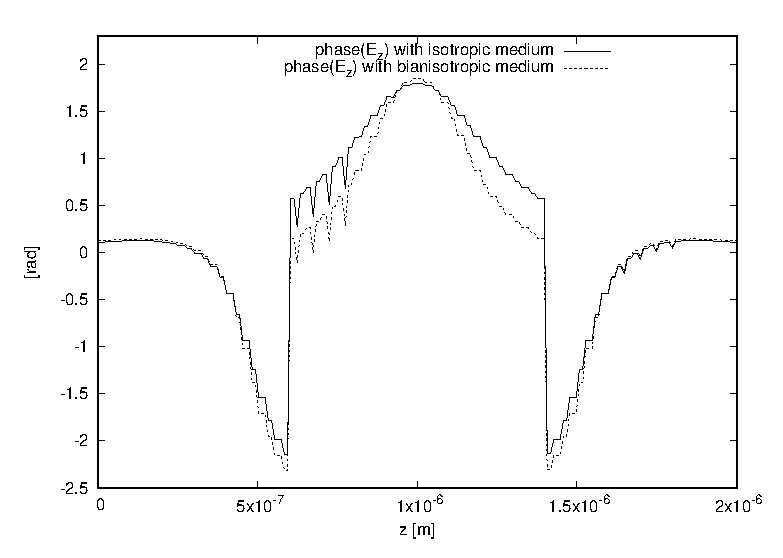
\includegraphics[width=\textwidth]{figure_kraft_pendry_along_z_phase_ez.eps}
\end{subfigure}
\caption{The magnitude and phase of the $z$ component of electric field along a line parallel to $z$ axis 
and passing though the center of gravity of the domain  for problem involving medium of Kraft et al. 
The plots for bianisotropic case using $\zeta_0 = -0.41$ is compared with 
the solution obtained in isotropic case using $\zeta_0 = 0$.}
\label{fi:kraft_pendry_ez_vs_z}
\end{figure}
